% Options for packages loaded elsewhere
% Options for packages loaded elsewhere
\PassOptionsToPackage{unicode}{hyperref}
\PassOptionsToPackage{hyphens}{url}
\PassOptionsToPackage{dvipsnames,svgnames,x11names}{xcolor}
%
\documentclass[
  british,
  a4paper,
]{article}
\usepackage{xcolor}
\usepackage{amsmath,amssymb}
\setcounter{secnumdepth}{-\maxdimen} % remove section numbering
\usepackage{iftex}
\ifPDFTeX
  \usepackage[T1]{fontenc}
  \usepackage[utf8]{inputenc}
  \usepackage{textcomp} % provide euro and other symbols
\else % if luatex or xetex
  \usepackage{unicode-math} % this also loads fontspec
  \defaultfontfeatures{Scale=MatchLowercase}
  \defaultfontfeatures[\rmfamily]{Ligatures=TeX,Scale=1}
\fi
\usepackage{lmodern}
\ifPDFTeX\else
  % xetex/luatex font selection
\fi
% Use upquote if available, for straight quotes in verbatim environments
\IfFileExists{upquote.sty}{\usepackage{upquote}}{}
\IfFileExists{microtype.sty}{% use microtype if available
  \usepackage[]{microtype}
  \UseMicrotypeSet[protrusion]{basicmath} % disable protrusion for tt fonts
}{}
\makeatletter
\@ifundefined{KOMAClassName}{% if non-KOMA class
  \IfFileExists{parskip.sty}{%
    \usepackage{parskip}
  }{% else
    \setlength{\parindent}{0pt}
    \setlength{\parskip}{6pt plus 2pt minus 1pt}}
}{% if KOMA class
  \KOMAoptions{parskip=half}}
\makeatother
% Make \paragraph and \subparagraph free-standing
\makeatletter
\ifx\paragraph\undefined\else
  \let\oldparagraph\paragraph
  \renewcommand{\paragraph}{
    \@ifstar
      \xxxParagraphStar
      \xxxParagraphNoStar
  }
  \newcommand{\xxxParagraphStar}[1]{\oldparagraph*{#1}\mbox{}}
  \newcommand{\xxxParagraphNoStar}[1]{\oldparagraph{#1}\mbox{}}
\fi
\ifx\subparagraph\undefined\else
  \let\oldsubparagraph\subparagraph
  \renewcommand{\subparagraph}{
    \@ifstar
      \xxxSubParagraphStar
      \xxxSubParagraphNoStar
  }
  \newcommand{\xxxSubParagraphStar}[1]{\oldsubparagraph*{#1}\mbox{}}
  \newcommand{\xxxSubParagraphNoStar}[1]{\oldsubparagraph{#1}\mbox{}}
\fi
\makeatother


\usepackage{longtable,booktabs,array}
\newcounter{none} % for unnumbered tables
\usepackage{calc} % for calculating minipage widths
% Correct order of tables after \paragraph or \subparagraph
\usepackage{etoolbox}
\makeatletter
\patchcmd\longtable{\par}{\if@noskipsec\mbox{}\fi\par}{}{}
\makeatother
% Allow footnotes in longtable head/foot
\IfFileExists{footnotehyper.sty}{\usepackage{footnotehyper}}{\usepackage{footnote}}
\makesavenoteenv{longtable}
\usepackage{graphicx}
\makeatletter
\newsavebox\pandoc@box
\newcommand*\pandocbounded[1]{% scales image to fit in text height/width
  \sbox\pandoc@box{#1}%
  \Gscale@div\@tempa{\textheight}{\dimexpr\ht\pandoc@box+\dp\pandoc@box\relax}%
  \Gscale@div\@tempb{\linewidth}{\wd\pandoc@box}%
  \ifdim\@tempb\p@<\@tempa\p@\let\@tempa\@tempb\fi% select the smaller of both
  \ifdim\@tempa\p@<\p@\scalebox{\@tempa}{\usebox\pandoc@box}%
  \else\usebox{\pandoc@box}%
  \fi%
}
% Set default figure placement to htbp
\def\fps@figure{htbp}
\makeatother



\ifLuaTeX
\usepackage[bidi=basic,shorthands=off]{babel}
\else
\usepackage[bidi=default,shorthands=off]{babel}
\fi
\ifLuaTeX
  \usepackage{selnolig} % disable illegal ligatures
\fi


\setlength{\emergencystretch}{3em} % prevent overfull lines

\providecommand{\tightlist}{%
  \setlength{\itemsep}{0pt}\setlength{\parskip}{0pt}}



 


\makeatletter
\@ifpackageloaded{tcolorbox}{}{\usepackage[skins,breakable]{tcolorbox}}
\@ifpackageloaded{fontawesome5}{}{\usepackage{fontawesome5}}
\definecolor{quarto-callout-color}{HTML}{909090}
\definecolor{quarto-callout-note-color}{HTML}{0758E5}
\definecolor{quarto-callout-important-color}{HTML}{CC1914}
\definecolor{quarto-callout-warning-color}{HTML}{EB9113}
\definecolor{quarto-callout-tip-color}{HTML}{00A047}
\definecolor{quarto-callout-caution-color}{HTML}{FC5300}
\definecolor{quarto-callout-color-frame}{HTML}{acacac}
\definecolor{quarto-callout-note-color-frame}{HTML}{4582ec}
\definecolor{quarto-callout-important-color-frame}{HTML}{d9534f}
\definecolor{quarto-callout-warning-color-frame}{HTML}{f0ad4e}
\definecolor{quarto-callout-tip-color-frame}{HTML}{02b875}
\definecolor{quarto-callout-caution-color-frame}{HTML}{fd7e14}
\makeatother
\makeatletter
\@ifpackageloaded{caption}{}{\usepackage{caption}}
\AtBeginDocument{%
\ifdefined\contentsname
  \renewcommand*\contentsname{Table of contents}
\else
  \newcommand\contentsname{Table of contents}
\fi
\ifdefined\listfigurename
  \renewcommand*\listfigurename{List of Figures}
\else
  \newcommand\listfigurename{List of Figures}
\fi
\ifdefined\listtablename
  \renewcommand*\listtablename{List of Tables}
\else
  \newcommand\listtablename{List of Tables}
\fi
\ifdefined\figurename
  \renewcommand*\figurename{Figure}
\else
  \newcommand\figurename{Figure}
\fi
\ifdefined\tablename
  \renewcommand*\tablename{Table}
\else
  \newcommand\tablename{Table}
\fi
}
\@ifpackageloaded{float}{}{\usepackage{float}}
\floatstyle{ruled}
\@ifundefined{c@chapter}{\newfloat{codelisting}{h}{lop}}{\newfloat{codelisting}{h}{lop}[chapter]}
\floatname{codelisting}{Listing}
\newcommand*\listoflistings{\listof{codelisting}{List of Listings}}
\makeatother
\makeatletter
\makeatother
\makeatletter
\@ifpackageloaded{caption}{}{\usepackage{caption}}
\@ifpackageloaded{subcaption}{}{\usepackage{subcaption}}
\makeatother
\usepackage{bookmark}
\IfFileExists{xurl.sty}{\usepackage{xurl}}{} % add URL line breaks if available
\urlstyle{same}
% fallback for those not using the hyperref driver hyperxmp:
\makeatletter
\@ifundefined{xmpquote}{\newcommand{\xmpquote}[1]{#1}}{}
\makeatother
\hypersetup{
  pdftitle={Nowcasting with mixed-frequency data and a shock module},
  pdfauthor={Carlos Galindo},
  pdflang={en-GB},
  colorlinks=true,
  linkcolor={blue},
  filecolor={Maroon},
  citecolor={Blue},
  urlcolor={Blue},
  pdfcreator={LaTeX via pandoc}}


\title{Nowcasting with mixed-frequency data and a shock module}
\usepackage{etoolbox}
\makeatletter
\providecommand{\subtitle}[1]{% add subtitle to \maketitle
  \apptocmd{\@title}{\par {\large #1 \par}}{}{}
}
\makeatother
\subtitle{A prototype that turns monthly signals and quarterly releases
into one running estimate, with a learned component for sudden shocks}
\author{Carlos Galindo}
\date{}
\begin{document}
\maketitle


\begin{tcolorbox}[enhanced jigsaw, arc=.35mm, bottomrule=.15mm, breakable, colback=white, colframe=quarto-callout-note-color-frame, left=2mm, leftrule=.75mm, opacityback=0, rightrule=.15mm, toprule=.15mm]

\vspace{-3mm}\textbf{At a glance}\vspace{3mm}

\begin{itemize}
\tightlist
\item
  \textbf{Question.} How can a monthly indicator set and a slow
  quarterly release be combined into one estimate of current growth that
  updates as each number arrives, and can a learned component help with
  sudden shocks?
\item
  \textbf{Approach.} A monthly latent-state model in which quarterly
  figures enter as averages of three monthly values, estimated with a
  Kalman filter. A machine-learning module supplies expected shocks
  together with their uncertainty.
\item
  \textbf{Finding.} The prototype runs end to end on simulated
  mixed-frequency data, with the quarterly figures correctly aligned and
  the shock module's uncertainty feeding the estimation. It has not yet
  been tested out of sample on real data.
\item
  \textbf{Why it matters.} The design keeps the linear core simple and
  auditable and treats the learned part as an optional, bounded add-on.
\end{itemize}

\end{tcolorbox}

\subsection{The question}\label{the-question}

Policy and markets want to know how the economy is doing now, but the
best measure of output arrives once a quarter and weeks late. In
between, monthly indicators arrive on different dates and cover
different periods. A nowcast is the attempt to turn that uneven stream
into a current estimate.

The obvious approaches fall short in two ways. Bridging by hand, which
averages monthly data into quarters and regresses on them, throws away
the timing of the information and cannot cope when some indicators are
published and others are not. And a purely linear model cannot
anticipate the sudden events, such as a policy announcement or an energy
price jump, that make nowcasting valuable in the first place.

This project is a prototype aimed at both gaps. It is a small,
transparent mixed-frequency model, plus a learned module whose only job
is to propose shocks that the linear core can absorb. The work was done
during a career break as an independent build. It was designed to be
audited line by line rather than to be impressive.

\subsection{Approach}\label{approach}

\textbf{A monthly state.} Everything is modelled at the highest
frequency in the problem, which is monthly. A small set of unobserved
monthly states, such as underlying activity, evolves through a linear
transition equation with an exogenous shock input. Monthly indicators
measure these states directly with noise.

\textbf{Quarterly figures as averages.} A quarterly observation is not a
monthly one. It is treated as an intermittent measurement that exists
only in the last month of each quarter. The cleanest version of this is
a strict aggregation restriction: the state is augmented with monthly
lags, so that the quarterly figure equals the average of the last three
monthly latent values. The prototype supports this strict form and a
conservative form that maps the quarterly figure onto the monthly latent
directly. The first is the more faithful of the two.

\textbf{The ragged edge.} Because the model sits at the monthly
frequency, an indicator that has not yet been published is simply a
missing measurement. The Kalman filter skips it and carries the state
forward, and when the number arrives the estimate updates. The same
mechanism handles quarterly figures, which are missing in two months out
of three. No special treatment of the ragged edge is needed.

\textbf{Estimation.} Parameters are estimated by
expectation-maximisation, with a floor on the shock variance and light
regularisation to keep the estimates stable in short samples.

\textbf{The shock module.} A supervised learning module is trained to
predict the exogenous shock from features. It returns a mean and a
covariance for each period, not only a point value. Three safeguards
keep it from damaging the core:

\begin{itemize}
\tightlist
\item
  predictions are clipped to a maximum shock magnitude;
\item
  if the module is missing or fails, the shock defaults to zero, so the
  model reverts to its plain linear form;
\item
  the module's reported uncertainty enters the variance of the shock
  input, so a weakly informative prediction counts for less in
  estimation.
\end{itemize}

An attribution layer, based on Shapley values, explains each period's
predicted shock in terms of its features. The contributions are then
projected through the input matrix onto the model's latent states, which
shows which inputs moved which state.

\textbf{Checks.} The design was held to a short list of acceptance
criteria: the augmented system must reproduce the plain one when the
optional pieces are off, estimation must stay stable across a grid of
settings and seeds, and every run must persist its settings so it can be
reproduced. A reality check on the output caught one real problem, in
which the quarterly series was misaligned with the monthly index and
arrived empty. It was fixed by aligning both on calendar periods.

\subsection{What the work shows}\label{what-the-work-shows}

The prototype's results are about design and behaviour, not about
forecast accuracy. It runs end to end on simulated mixed-frequency data,
which includes monthly states and indicators, daily series aggregated to
monthly, and quarterly figures aligned at quarter-end. The quarterly
series is correctly populated after the alignment fix. The model's
parameters are estimated and saved, and the report shows both the
monthly and the quarterly series.

The figures below use simulated data built to share the structure of the
problem. They illustrate how the method behaves.

\begin{figure}

\centering{

\pandocbounded{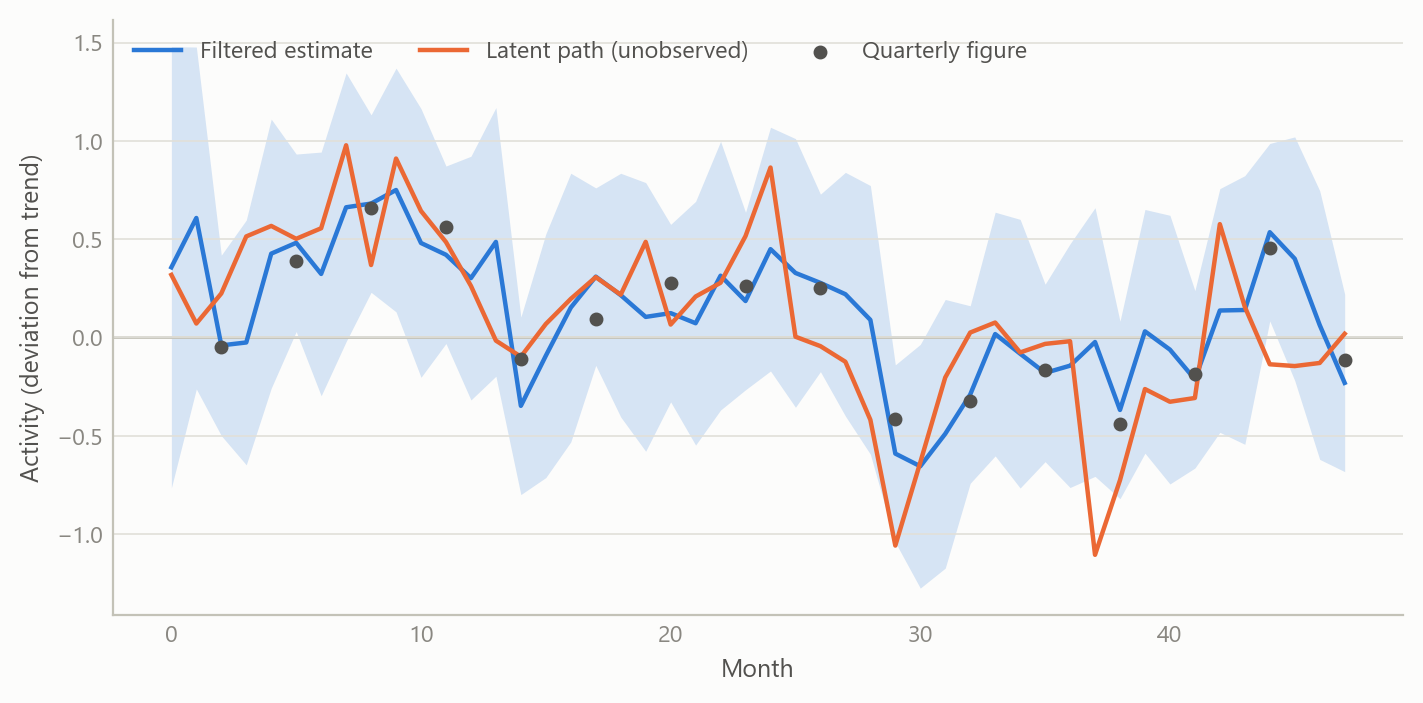
\includegraphics[keepaspectratio]{index_files/figure-latex/fig-ragged-output-1.png}}

}

\caption{\label{fig-ragged}A monthly latent activity path, noisy
quarterly averages observed at quarter-end, and the filtered estimate
with its band (simulated data).}

\end{figure}%

\begin{figure}

\centering{

\pandocbounded{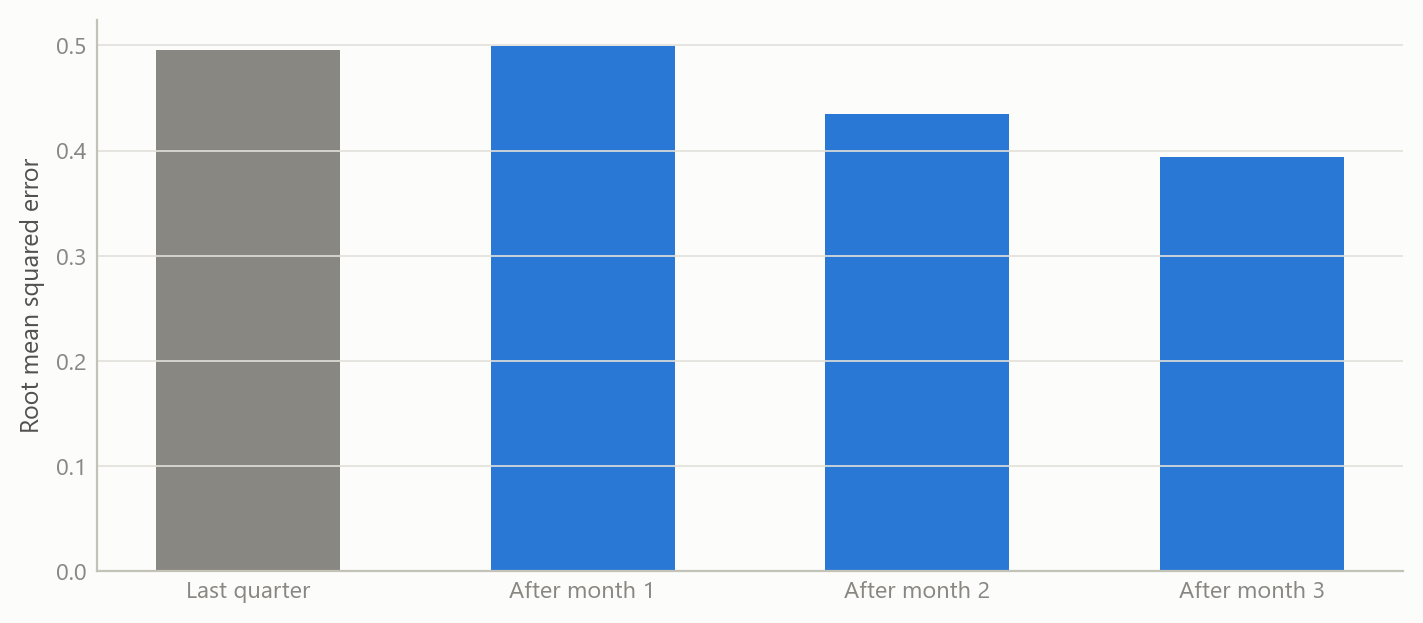
\includegraphics[keepaspectratio]{index_files/figure-latex/fig-vintage-output-1.png}}

}

\caption{\label{fig-vintage}Average error of the current-quarter nowcast
by how many months of data are in, against a naive benchmark (simulated
data).}

\end{figure}%

\begin{figure}

\centering{

\pandocbounded{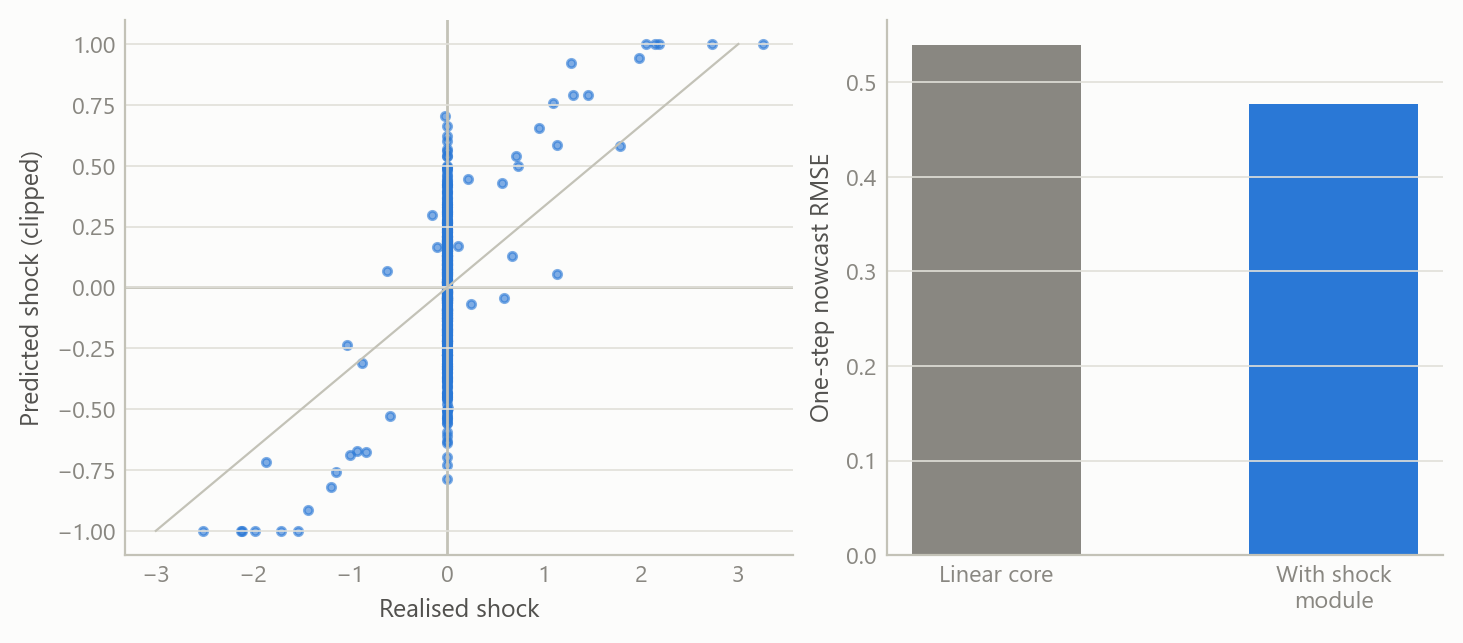
\includegraphics[keepaspectratio]{index_files/figure-latex/fig-shock-output-1.png}}

}

\caption{\label{fig-shock}Left: shocks predicted by the learned module
against realised shocks, clipped at a bound. Right: nowcast error with
and without the module (simulated data).}

\end{figure}%

The first figure shows the mechanism: quarterly figures pin down the
three-month average, monthly indicators fill in the path between them,
and the band narrows when information arrives. The second shows the
pattern a nowcast should have, with error falling as each month of data
comes in. The third shows the shock module's role, which is to cut error
in the periods after a sudden event while its clipping keeps any single
prediction bounded. These patterns are properties of the design, shown
on simulated data. They are not measured accuracy.

\subsection{Insights}\label{insights}

\begin{enumerate}
\def\labelenumi{\arabic{enumi}.}
\tightlist
\item
  \textbf{Treat the quarterly figure as a restriction, not a variable to
  be interpolated.} Writing it as the average of three monthly states
  lets one model handle both frequencies, and the missing-data logic of
  the filter does the rest.
\item
  \textbf{Keep the learned part outside the core.} The shock module is
  optional, bounded and replaceable. If it fails, the model degrades to
  a plain linear nowcast, not to nonsense.
\item
  \textbf{Pass uncertainty, not only predictions.} A shock forecast with
  a covariance lets estimation weigh a weak prediction lightly. A point
  forecast does not.
\item
  \textbf{Attribution belongs in the state space.} Mapping feature
  contributions through the input matrix onto the latent states makes an
  opaque predictor answer the question a macroeconomist would ask: which
  state moved, and why.
\item
  \textbf{Alignment bugs are silent.} Misaligned calendar periods
  produce empty quarterly columns, not errors. A minimal reality check
  on the output, not only on the code, found it.
\end{enumerate}

\subsection{Scope and next steps}\label{scope-and-next-steps}

The current status is a working prototype. It has not been evaluated out
of sample on real data, so it makes no claim about forecast accuracy or
about whether the shock module adds value in practice. The module was
trained and exercised on simulated data only. The model is linear in its
core and has a single latent-factor flavour, with no treatment of data
revisions or of publication-date calendars.

Three steps would turn it into evidence. First, assemble a real-time
vintage dataset for one economy and run a pseudo-real-time test by
information vintage against a simple benchmark. Second, train the shock
module on genuine event features and report its cross-validated error,
then test whether it improves the nowcast. Third, add a revision model
so that early releases are treated as noisy measurements of later ones.

\subsection{About the evidence}\label{about-the-evidence}

The work is an independent prototype built during a career break, in
2025, and it was documented through design notes, a staged plan with
acceptance tests, and generated reports. It was run on simulated
mixed-frequency data of a few monthly states, daily series aggregated to
months, and quarterly figures. It has no real-data results. All figures
on this page are simulated.

Figures and tables marked \emph{simulated} are generated from simulated
data built to share the structure of the analysis (its variables,
horizons and frequencies). They show how each method works and what its
output looks like. Results stated in the text, and figures that give a
source, are the project's own. Methods are described at the level of a
methods section. Code and data pipelines are not reproduced here.




\end{document}
